\documentclass[11pt]{article}
\usepackage{../EllioStyle}
\usepackage{listings}

\definecolor{codegreen}{rgb}{0,0.6,0}
\definecolor{codegray}{rgb}{0.5,0.5,0.5}
\definecolor{codepurple}{rgb}{0.58,0,0.82}
\definecolor{backcolour}{rgb}{0.95,0.95,0.92}

\graphicspath{ {imgs/} }

\title{Homework 1}
\author{Elliott Pryor}
\date{6 September 2023}

\rhead{Homework 1}


\begin{document}
\maketitle

\problem{1}

Consider the system shown in Figure \ref{fig:1-1}. Derive the expression for y(t) in
terms of $y(0)$, $\dot{y}(0)$ and $f(t)$.

\begin{figure}[h] 
    \centering
    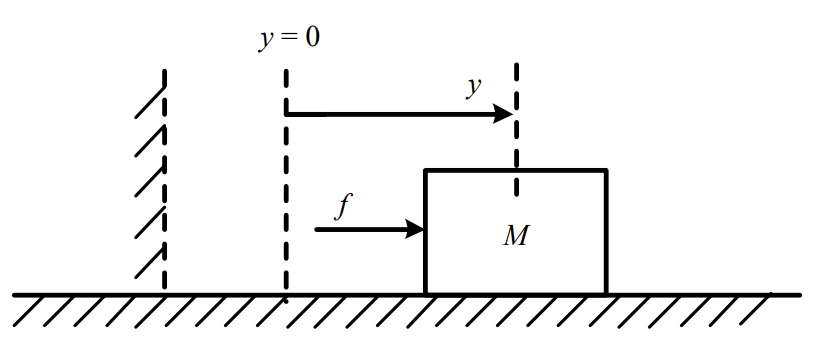
\includegraphics[width=0.55 \linewidth]{fig11.png}
    \caption{System for Problem 1,2}
    \label{fig:1-1}
\end{figure}

\soln



\problem{2}

Consider the system shown in Figure \ref{fig:1-1}. Calculate an open loop control $f(t)$
to bring $y(t)$ from $y(0) = y_0 \neq 0$ and $\dot{y}(0) = 0$ to $y(1) = 0$ and $\dot{y}(1) = 0$. 
If $M$ is reduced to $0.9M$, under the same $f(t)$, what will $y(1)$ be?

\soln


\problem{3}

Describe how you usually adjust the shower water temperature you are
comfortable with. What type of feedback do you think you are applying? What are the
actuator and sensor?

\soln




\problem{4}

Identify a feedback control system that is not discussed in this chapter and
describe how feedback works in the system.

\soln




\problem{5}

Consider the toilet water tank, shown in Figure \ref{fig:16}. One way to reduce the
amount of water used for each flush is put a rock inside the water tank. Would this cause
the water level to rise higher when the fill valve is closed off? Give your reason.

\begin{figure}[h] 
    \centering
    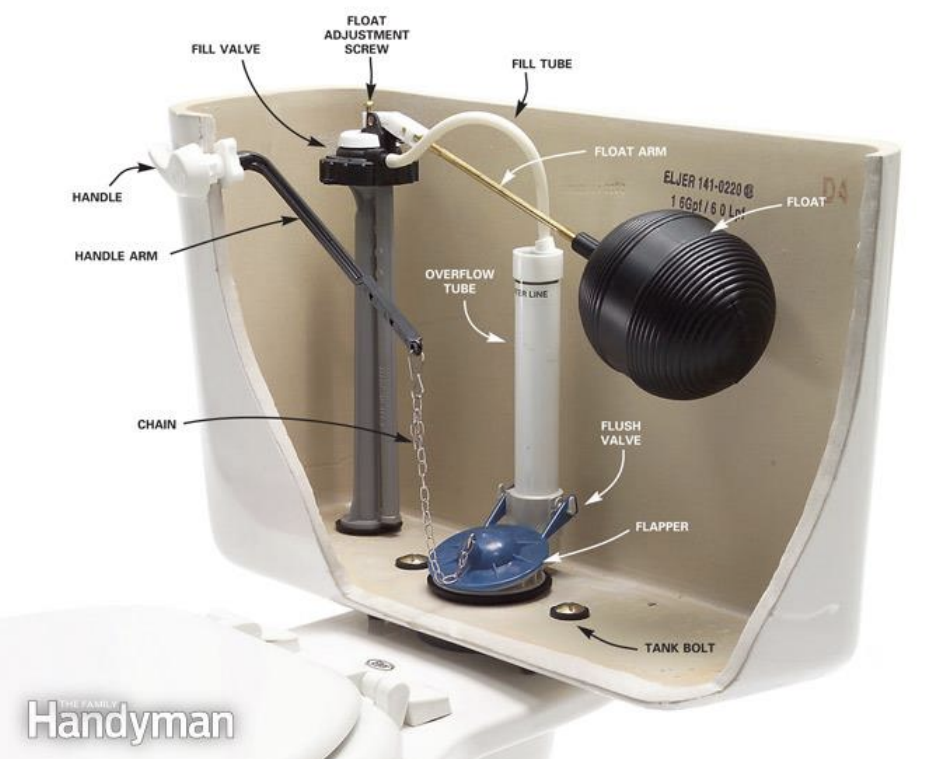
\includegraphics[width=0.55 \linewidth]{fig16.png}
    \caption{System for problem 5}
    \label{fig:16}
\end{figure}

\soln




\problem{6}

How would you set the desired water level in the toilet water tank, shown in
Figure \ref{fig:16}, and the desired shaft rotation speed in the Watt steam engine, shown in Fig. \ref{fig:watt}?

\begin{figure}[h]
    \centering
    \begin{subfigure}[b]{0.45\textwidth}
        \centering
        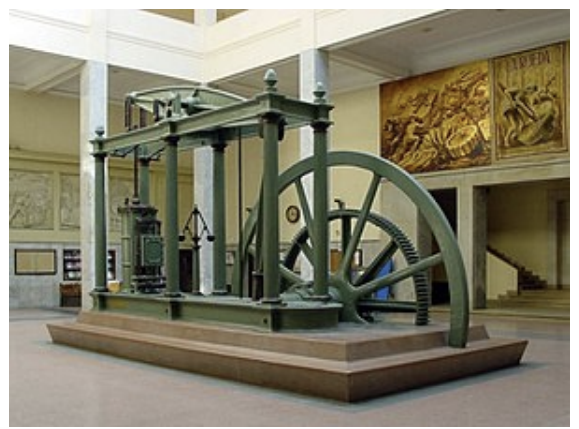
\includegraphics[width=\textwidth]{fig17}
        \label{fig:w1}
    \end{subfigure}
    \hfill
    \begin{subfigure}[b]{0.45\textwidth}
        \centering
        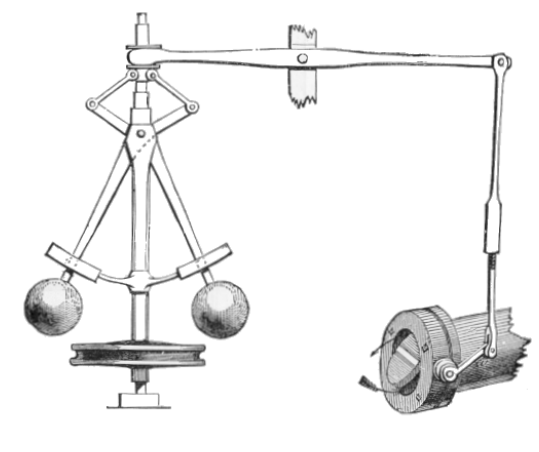
\includegraphics[width=\textwidth]{fig18}
        \label{fig:w2}
    \end{subfigure}
    \caption{Watt engine diagram}
    \label{fig:watt}
\end{figure}


\soln

\end{document}